\chapter{Video Generation}\label{ch:results}

    In this chapter we combine the methods from the previous chapters. We also elaborate on some further preprocessing during the generation of videos. Finally we do our best to provide some results on paper.

    \section{Generating videos}
        
        Theoretically we can generate videos with each possible combination of extracted features and trained generators.

        \begin{itemize}
            \item how did we generate images from the trained nets?
            \item maybe also discuss/display intermediate results? (genre classification, autoencoder, single generated images)
        \end{itemize}

    \section{Ensuring smooth transitions}
        
        \begin{itemize}
            \item smoothing?
            \item what did we do to smoothen the video?
            \item smoothing --> talk about the movement through feature space when producing a video from song
        \end{itemize}

    \section{Results}

        Actual example videos can be downloaded and / or generated as described in the next chapter.

        \begin{figure}[ht]
            \centering
            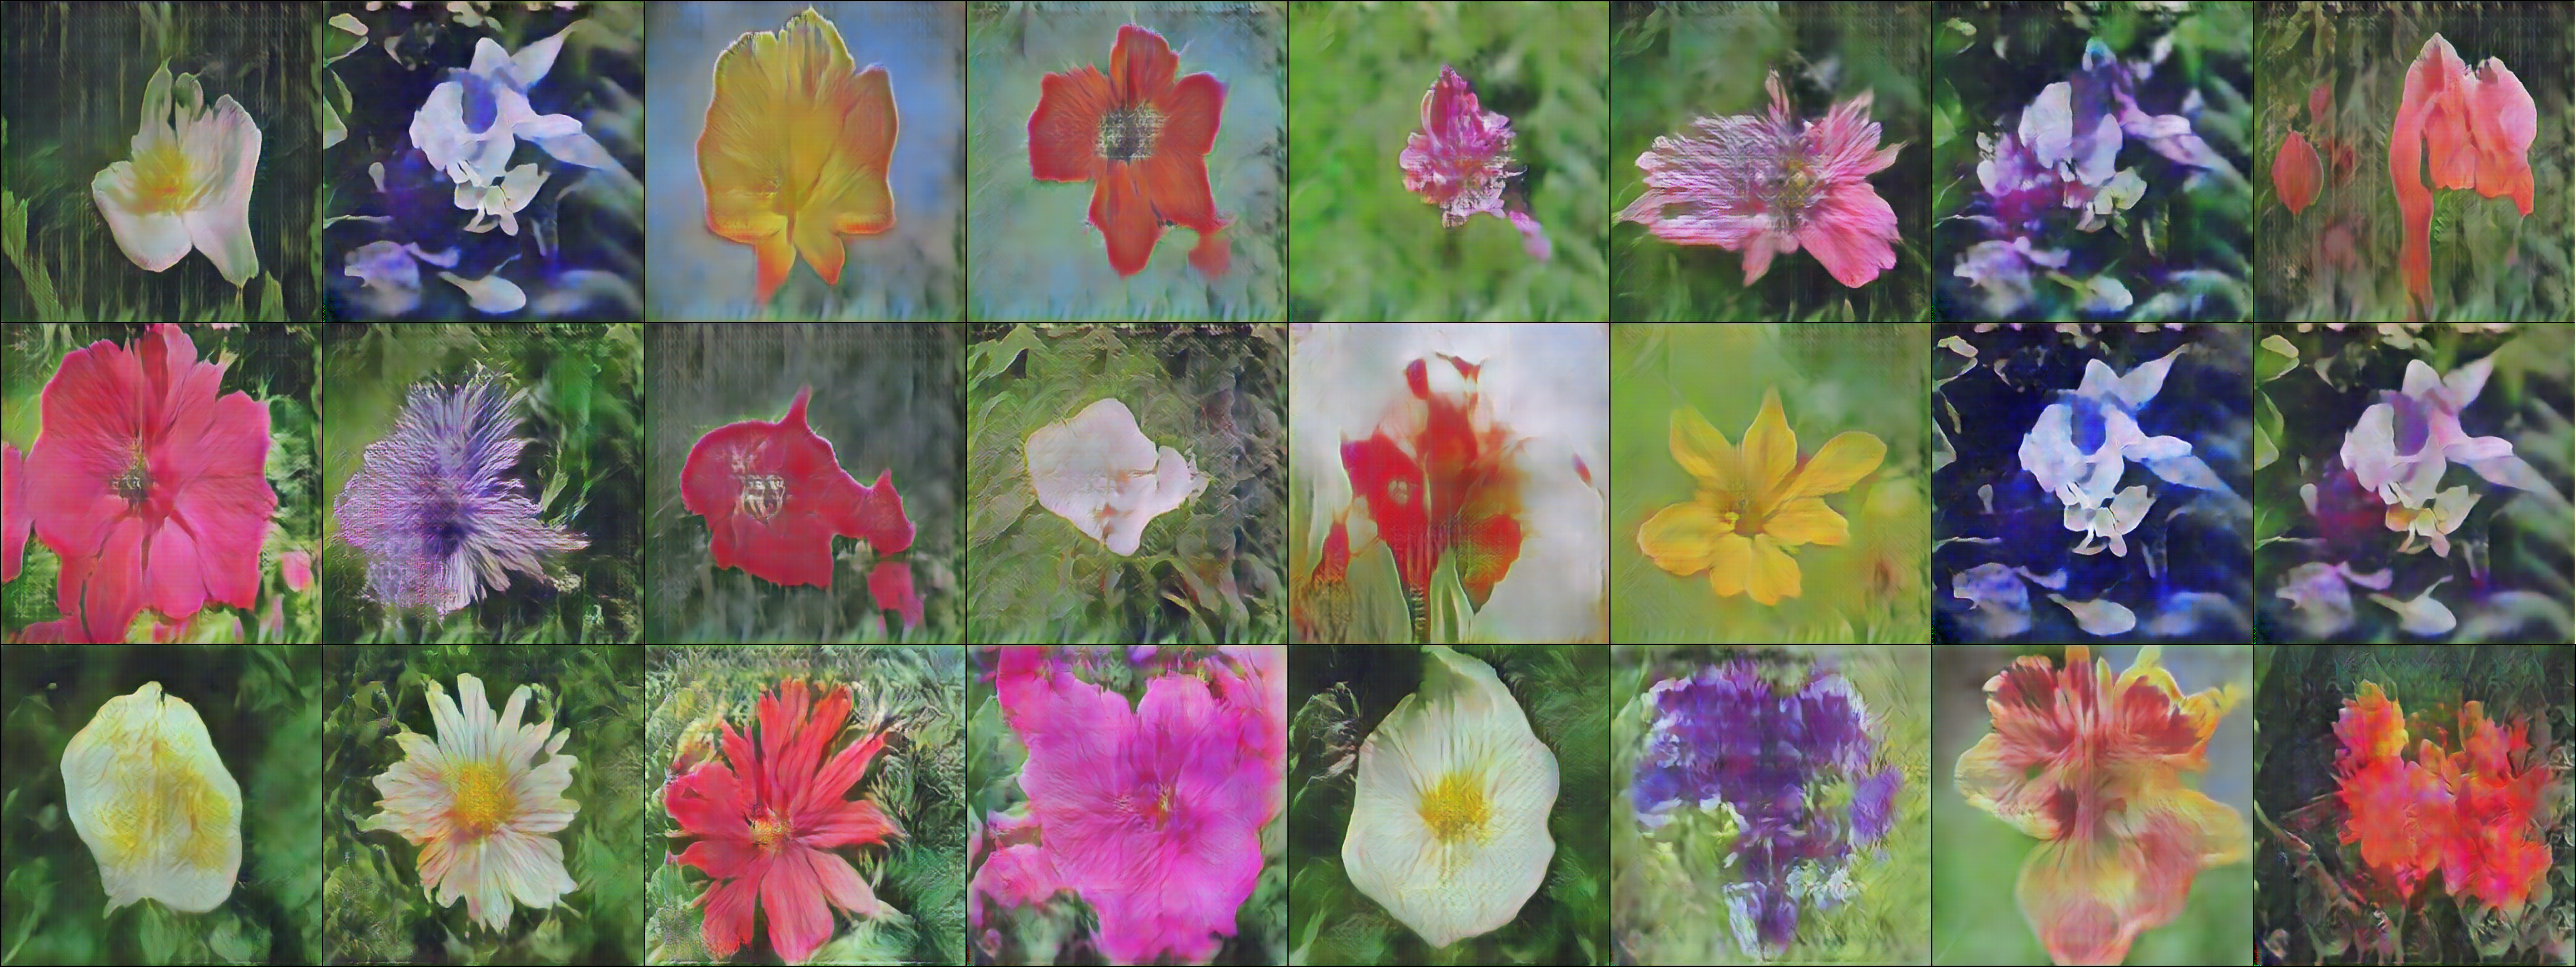
\includegraphics[width=.94\textwidth]{images/fake_samples_not_cherry_picked}
            \caption[not used]
            {
                \textbf{\TODO{do}.}
            }
            \label{fig:dcgan_samples}
        \end{figure}

        \begin{figure}[ht]
            \centering
            \fbox{
                \includegraphics[width=.94\textwidth]{images/video_on_paper}
            }
            \caption[not used]
            {
                \textbf{\TODO{do}.}
            }
            \label{fig:video}
        \end{figure}

        \begin{itemize}
            \item display the stuff that was on the poster? in an attempt to put a video on paper
        \end{itemize}
